\documentclass[letterpaper, onecolumn, 11pt]{report}
\usepackage[utf8]{inputenc}
%\usepackage[spanish]{babel}
\usepackage{amsmath}
\usepackage{graphicx}
%\usepackage{txfonts} %bkn
\usepackage{physics}
\usepackage{wrapfig}
\usepackage{hyperref}
\usepackage{marginnote}
\usepackage{caption}
\usepackage{amsfonts}
%\usepackage{draculatheme} %Agregar draculatheme.sty  al directorio del proyecto LaTeX
%\spanishdecimal{.}
\usepackage{hyperref}
\usepackage{marginnote}
\hypersetup{colorlinks=true, linkcolor=red}

\renewcommand*{\marginnotevadjust}{-0.1cm}
\renewcommand*{\marginfont}{\footnotesize}
\usepackage[right=4.5cm,left=2cm,top=3cm,bottom=3.0cm]{geometry}
\begin{document}
\sffamily
\begin{center}

\

\vspace{6.5cm}

\rule{15cm}{0.1cm}

\vspace{1.5cm}

{\huge \textsc{\textbf{Quantum Mechanics}}}

\vspace{1.5cm}

\rule{15cm}{0.1cm}

Diez B. Borja
\vspace{1.5cm}

\today

\end{center}
%\title{\Huge\textbf{{Quantum Mechanics}}}
\author{Diez B. Borja}
%\maketitle
\tableofcontents
\input{cap/the-wave-function.tex}
\chapter{Time-Independent Schrodinger Equation}
\section{Stationary States}
Wa talked a lot about the wave function, and how you use it to calculare various quantities of interest. But, how do get $\Psi(x,t)$ in the first place? We need to solce the Schrodinger equation,
\begin{equation}\label{2.1}
	i\hbar\pdv{\Psi}{t}=-\frac{\hbar^2}{2m}\pdv[2]{\Psi}{x}+V\Psi
\end{equation}
for a specified potential\footnote{It is tiresome to keep saying "potential energy function", so most people jus call $V$ the "potential", even though this invites occasional confusion with electric potencial, which is actually potential energy per unit charge.} $V(x,t)$. In this chapter (and most of this book) I shall assume that $V$ is \textit{independent} of $t$. In that case the Schrodinger equation can be solved by the method of \textbf{separation of variables}: We look for solutions that are simple \textit{products},
\begin{equation}\label{2.2}
	\Psi(x,t)=\psi(x)\varphi(t)
\end{equation}
where $\psi$ is a function of $x$ alone, and $\varphi$ is a function of $t$ alone. 

For separable solutions we have
\begin{equation*}
	\pdv{\Psi}{t}=\psi\dv{\varphi}{t},\qquad \pdv[2]{\Psi}{x}=\dv[2]{\psi}{x}\varphi
\end{equation*}
(\textit{ordinaty} derivatives, now), and Schrodinger equation reads
\begin{equation}
	i\hbar\dv{\varphi}{t}=-\frac{\hbar^2}{2m}\dv[2]{\psi}{x}\varphi + V\psi\varphi
\end{equation}
Or, dividing through by $\psi\varphi$:
\begin{equation}\label{2.3}
	i\hbar\frac{1}{\varphi}\dv{\varphi}{t}=-\frac{\hbar^2}{2m}\frac{1}{\psi}\dv[2]{\psi}{x}+V
\end{equation}

Now, the left side is a function of $t$ alone, and the right side is a function of $x$ alone\footnote{Note that this would not be true if $V$ were a function of $t$ as well as $x$.}. The only way this can possibly be true is if both sides are in fact \textit{constant} -- otherwise, by varying $t$, I could change the left side without touching the right side, and the two would no lonegr equal. For reasons that will appear in a moment, we shall call the separation constan $E$. Then
\begin{equation*}
	i\hbar\frac{1}{\varphi}\dv{\varphi}{t}=E
\end{equation*}
or
\begin{equation*}\label{2.4}
	\dv{\varphi}{t}=-\frac{iE}{\hbar}\varphi
\end{equation*}
and
\begin{equation}
	-\frac{\hbar^2}{2m}\frac{1}{\psi}\dv[2]{\psi}{x}+V=E
\end{equation}
or
\begin{equation}\label{2.5}\marginnote{Time-independent Schrodinger equation}
	\boxed{-\frac{\hbar^2}{2m}\dv[2]{\psi}{x}+V\psi=E\psi}
\end{equation}
Separation of variables hs turned a \textit{partial} differential equation into \textit{two ordinary} differential equations (\ref{2.4}) and (\ref{2.5}). The first, (\ref{2.4}) is easy to solve (just multiply through by $\dd t$ and integrate); the general solution is $C\exp(-iEt/\hbar)$, but we might as well absorb the constant $C$ into $\psi$ (since the quantity of interest is the product $\psi\varphi$). Then
\begin{equation}\label{2.6}
	\varphi(t)=e^{-iEt/\hbar}
\end{equation}
The second equation (\ref{2.5}) is called the \textit{time-independent Schrodinger equation} we can go further with it until the potencial $V(x)$ is specified.

The rest of thus chapter will be devoted to solving the time-independent Schrodinger equation, fot a variety of simple potentials. But before I get to that you have every right ask: What's so great about separable solutions? After all, most solutions so the (time dependent) Schrodinger equation do not take the form $\psi(x)\varphi(t)$. I offer three answers--two of them physical, and one mathematical:
\begin{enumerate}
	\item They are \textbf{stationaty states}. Although the wave function itself,
\begin{equation}\label{2.7}
	\Psi(x,t)=\psi(x)e^{-iEt/\hbar}
\end{equation}
does (obviously) depende on $t$, the \textit{probability density},
\begin{equation}\label{2.8}
	|\Psi(x,t)|^2=\Psi^*\Psi=\psi^*e^{+iEt/\hbar}\psi e^{-iEt/\hbar}=|\psi(x)|^2
\end{equation}
does not--the time-dependence cancels out\footnote{For normalizable solutions, $E$ must be real}. The same thing happens in calculate the expectation value of any dynamil variable; (\ref{1.36}) reduces to
\begin{equation}\label{2.9}
	<Q(x,p)>=\int\psi^*Q\left(x,\frac{\hbar}{i}\frac{\dd}{\dd x}\right)\psi\dd x
\end{equation}
\textit{Every expectation value is constant in time}; we might as well drop the factor $\varphi(t)$ altogether, and simply use $\psi$ in place of $\Psi$. In particular, $<x>$ is constant, and hence $<p>=0$ (See (\ref{1.33})). Nothing ever happens in a stationary state.

\item They are states of \textit{definite total energy}. In classical mechanics, the total energy (kinetic plus pontential) is called the \textbf{Hamiltonian}:
	\begin{equation}\label{2.10}
	H(x,p)=\frac{p^2}{2m}+V(x)
\end{equation}
The corresponding Hamiltonian \textit{operator}, obtained by the canonical substitution $p\to (\hbar/i)(\partial /\partial x)$, is therefore\footnote{Whenever confusion might arise. I'll put a "hat" on the operator, to distinguish it from the dynamical variable it represents.}
\begin{equation}\label{2.11}
	\hat{H}=-\frac{\hbar^2}{2m}\frac{\partial^2}{\partial x^2}+V(x)
\end{equation}
Thus the time-independent Schrodinger equation (\ref{2.5}) can be written
\begin{equation}\label{2.12}
	\hat{H}\psi=E\psi
\end{equation}
and the expectation value of the total energy is
\begin{equation}\label{2.13}
	<H>=\int\psi^*\hat{H}\psi\dd x=E\int |\psi|^2\dd x=E\int |\Psi|^2\dd x=E
\end{equation}
(Notice that the normalization of $\Psi$ entails the normalization of $\psi$.) Moreover,
$$\hat{H}^2\psi=\hat{H}(\hat{H}\psi)=\hat{H}(E\psi)=E(\hat{H}\psi)=E^2\psi$$ and hence $$<H^2>=\int\psi^*\hat{H}^2\psi\dd x=E^2\int|\psi|^2\dd x=E^2$$ So the variance of $H$ is 
\begin{equation}\label{2.14}
	\sigma_H^2=<H^2>-<H>^2=E^2-E^2=0
\end{equation}
But remember, if $\sigma=0$, then every member of the sample must share the same value (the distribution has zero spread). \textit{Conclusion}: A separable solution has the property that \textit{every measurement of the total energy is certain to return the value $E$}.

\item The general solution is a \textbf{linear combiantion} of separable solutions. As we're about to discover, the time-independent Schrodinger equation (\ref{2.5}) yields an infinite collection of solution ($\psi_1(x), \psi_2(x),...$),  each with its assocaites value of the reparation constant ($E_1, E_2, ...$); thus there is a different wave function for each \textbf{allowed energy}:
	$$\Psi_1(x,t)=\psi_1(x)e^{-iE_1t/\hbar},\qquad \Psi_2(x,t)=\psi_2(x)e^{-iE_2t/\hbar}, ...$$ Now the time-dependent Schrodinger equation (\ref{2.1}) has the property that any linear combination\footnote{A \textbf{linear combination} of the functions $f_1(z), f_z(z),...$ is an expression of the form $$f(z)=c_1f_1(z)+c_2f_2(z)+\cdots$$ where $c_1,c_2,...$ are any (complex) constants.} of solutions is itself a solution. Once we have found the separable solutions, then, we can immediately construct a much more general solution, on the form
\end{enumerate}
	\begin{equation}\label{2.15}
	\Psi(x,t)=\sum_{n=1}^\infty c_n\psi_n(x)e^{-iE_nt/\hbar}
\end{equation}
It so happens that \textit{every} solution to the (time-dependent) Schrodinger equation can be written iun this form --it is simply a matter if finding the tight constants ($c_1,c_2,...$) so as to fit the initial conditions for the problem at hand.

Let me recapitulate, from a somewhat different persperctive. Here's the generic problem: You're given a (time-independent) potencial $V(x)$ and the starting wave function $\Psi(x,0)$; your job is to find the wave function, $\Psi(x,t)$, for any subsequent time $t$. To do this you must solve the (time-dependent) Schrodinger equation (\ref{2.1}); this yields, in general, an infinite set of solutions ($\psi_1(x),\psi_2(x),...$), each with its own assocaited energy ($E_1,E_2,...$). To fit $\Psi(x,0)$ you write down the general linear combination of these solutions:
\begin{equation}\label{2.16}
	\Psi(x,0)=\sum_{n=1}^\infty c_n\psi_n(x)
\end{equation}
the miraacle os that you can \textit{always} match the specified initial state by appropiate choice of the constants $c_1,c_2,...$. To construct $\Psi(x,t)$ you simply tack onto each term its characteristic time dependence, $\exp(-iE_nt/\hbar)$:
\begin{equation}\label{2.17}
	\boxed{\Psi(x,t)=\sum_{n=1}^\infty c_n\psi_n(x)e^{-iE_nt/\hbar}=\sum_{n=1}^\infty c_n\Psi_n(x,t)}
\end{equation}
The separable solutions themselves,
\begin{equation}\label{2.18}
	\Psi_n(x,t)=\psi_n(x)e^{-iE_nt/\hbar}
\end{equation}
are \textit{stationary} states, in the sense that all probabilities and expectation values are independent of time, but this property is emphatically \textit{not} shared by the general solution (\ref{2.17}); the enrgies are different, for different stationary states, and the exponentials do not cancel, when you calculate $|\Psi|^2$.

\section{The Infinite Square Well}
\begin{figure}[h!]
	\begin{center}
		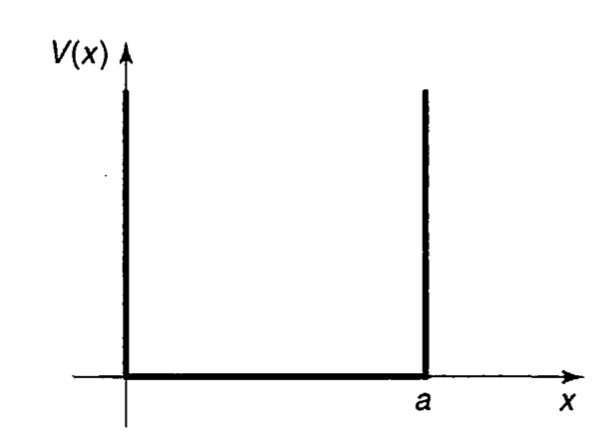
\includegraphics[scale=0.5]{fig/01.png}
		\caption{The infinte square well potential (\ref{2.19})}
		\label{fig:2.1}
	\end{center}	
\end{figure}

Suppose
\begin{equation}\label{2.19}
	V(x)=\left\{\begin{array}{lc}
		0&,0\leq x\leq a\\ \infty & \mbox{,otherwise}\end{array}
		\right.
\end{equation}
Fig. (\ref{fig:2.1}). A particle in this potential is completely free, except at two ends ($x=0$ and $x=a$), where an infinte force prevents it from escaping.

\textit{Outside} the well, $\psi(x)=0$ (the probability of findig the particle there is zero) \textit{Inside} the well, where $V=0$, the time-independent Schrodinger equation (\ref{2.5}) reads
\begin{equation}\label{2.20}
	-\frac{\hbar^2}{2m}\dv[2]{\psi}{x}=E\psi
\end{equation}
or
\begin{equation}\label{2.21}
	\dv[2]{\psi}{x}=-k^2\psi,\qquad \mbox{where } k\equiv\frac{\sqrt{2mE}}{\hbar}
\end{equation}
(By writinf it in this way, I have tacitly assumed that $E\geq 0$.) Equation (\ref{2.21}) is the classical \textbf{simple harmonic oscilaltor} equation; the general solution is
\begin{equation}\label{2.22}
	\psi(x)=A\sin kx + B\cos kx
\end{equation}
where $A$ and $B$ are arbitraty constants. Tipically, these constants are fixed by the \textbf{boundary conditions} of the problem. What are the appropiate boundary conditions for $\psi(x)$? Ordinatily, both $\psi$ and $\dd \psi/\dd x$ are continuous, but where the potential goes to infinity only the first of these applies.

Continuity of $\psi(x)$ requieres that
\begin{equation}\label{2.23}
	\psi(0)=\psi(a)=0
\end{equation}
so as to join onto the solution outisde the well. What does this tell us about $A$ and $B$? Well,
\begin{equation*}
	\psi(0)=A\sin 0+B\cos 0=B
\end{equation*}
so $B=0$, and hence
\begin{equation}\label{2.24}
	\psi(x)=A\sin kx
\end{equation}
Then $\psi(a)=A\sin ka$, so either $A=0$ (in which case we're left with the trivial --non-normalizable--solution $\psi(x)=0$), or else $\sin ka=0$, which means that
\begin{equation}\label{2.25}
	ka = 0,\pm \pi,\pm 2\pi,\pm 3\pi,...
\end{equation}
But $k=0$ is no good (again, that would imply $\psi(x)=0$),and the negative solutions give nothing new, since $\sin(-\theta)=-\sin(\theta)$ andw e can absorb the minus sign into $A$. So the \textit{distinct} solutions are
\begin{equation}\label{2.26}
	k_n=\frac{n\pi}{a},\qquad \mbox{with } n=1,2,3,...
\end{equation}
Curiously, the boundary condition at $x=a$ does not determine the constant $A$, but rather the constant $k$, and hence the possible values of $E$:
\begin{equation}\label{2.27}\marginnote{Possible values of $E$}
	\boxed{E_n=\frac{\hbar^2k_n^2}{2m}=\frac{n^2\pi^2\hbar^2}{2ma^2}}
\end{equation}
In radical contrast to the classical case, a quantum particle in the infinite square well cannot have just any old energy--it has be one of these special \textbf{allowed} values\footnote{Notice that the quantization of energy emerged as a rather technical consequence of the boudnary conditions on solutions to the time-independent Schrodinger equation}. To find $A$ we normalize $\psi$:
$$\int_a^{a}|A|^2\sin^2(kx)\dd x=|A|^2\frac{a}{2}=1,\qquad \mbox{ so  }|A|^2=\frac{2}{a}$$ 
This only determines the ,agnitude if $A$,  but it is simples to pick the positive real root: $A=\sqrt{2/a}$ (the phase of $A$ carries no physical significance anyway). Inside the well, the, the solutions are
\begin{equation}\label{2.28}
	\boxed{\psi_n(x)=\sqrt{\frac{2}{a}}\sin\left(\frac{n\pi}{a}x\right)}
\end{equation}
As a collection, the functions $\psi_n(x)$ have some interesting and important properties:
\begin{enumerate}
	\item They are alternately \textbf{even} and \textbf{odd}, with respecto to the center of the well: $\psi_1$ is even, $\psi_2$ is odd, $\psi_3$ is even,  and so on.
	\item 
		As you go up in energy, each successive state has one more \textbf{node} (zero-crossing): $\psi_1$ has one (the end points don't count), $\psi_4$ has one, $\psi_3$ has two, and so on.
	\item They are mutually \textbf{orthogonal}, in the sense that
		\begin{equation}\label{2.29}
	\int\psi_m(x)^*\psi_n(x)\dd x=0
\end{equation}
whenever $m\neq n$
We can combine orthogonality and normalization into a single satatement\footnote{In this case the $\psi$'s are real, so the * on $\psi_m$ is unnecessary, but for future purposes it's a good idea to get the habir of putting it there.}:
\begin{equation}\label{2.30}
	\boxed{\int\psi_m(x)^*\psi_n(x)\dd x=\delta_{mn}}
\end{equation}
We say that the $\psi$'s are \textbf{orthonormal}.'
\item They are \textbf{complete}, in the sense that any other function, $f(x)$, can be expressed as a linear combination of them:
	\begin{equation}\label{2.32}
	f(x)=\sum_{n=1}^\infty c_n\psi_n(x)=\sqrt{\frac{2}{a}}\sum_{n=1}^\infty c_n\sin\left(\frac{n\pi}{a}x\right)
\end{equation}
\end{enumerate}
(\ref{2.32}) is nothing but the \textbf{Fourier series} for $f(x)$, and the fact that any function can be expanded in this way is sometimes called \textbf{Dirichlet's theorem} 
The coefficients $c_n$ can be evaluated--for a given $f(x)$--by a method I call \textbf{Fourier's trick}, which beautifully exploits the orthonormality of $\{\psi_n\}$: Multiply both sides of (\ref{2.32}) by $\psi_m(x)^*$, and integrate
\begin{equation}\label{2.33}
	\psi_m(x)^*f(x)\dd x=\sum_{n=1}^\infty c_n\int\psi_m(x)^*\psi_n(x)\dd x=\sum_{n=1}^\infty c_n\delta_{nm}=c_n
\end{equation}
Thus the $n$th coefficient in the expansion of $f(x)$ is 
\begin{equation}\label{2.34}
	\boxed{c_n=\int\psi_n(x)^*f(x)\dd x}
\end{equation}
Completeness holds for all the potentials you are likely to encounter, but the proofs tens to be nasty and laborious.

The stationary states (\ref{2.18}) of the infinite square well are evidently
\begin{equation}\label{2.35}
	\Psi_n(x,t)=\sqrt{\frac{2}{a}}\sin\left(\frac{n\pi}{a}x\right)e^{-i(n^2\pi^2\hbar/2ma^2)t}
\end{equation}
I claimed (\ref{2.17}) that the most general solution to the (time-dependent) Schrodinger equation is a linear combinations of stationary states:
\begin{equation}\label{2.36}
	\Psi(x,t)=\sum_{n=1}^\infty c_n\sqrt{\frac{2}{a}}\sin\left(\frac{n\pi}{a}x\right)e^{-i(n^2\pi^2\hbar/2ma^2)t}
\end{equation}
It remaisn only for me to demosntrate that I can fit any prescribed initial wave fucntion, $\Psi(x,0)$, by appropiate choice of the coefficients $c_n$:
\begin{equation*}
	\Psi(x,0)=\sum_{n=1}^\infty c_n\psi_n(x)
\end{equation*}
The completeness of the $\psi$'s guarantees that I can always express $\Psi(x,0)$ in this way, and their orthonormality licenses the use of Fourier's trick to determine the actual coefficients:
\begin{equation}\label{2.37}
	c_n=\sqrt{\frac{2}{a}}\int_a^{a}\sin\left(\frac{n\pi}{a}x\right)\Psi(x,0)\dd x
\end{equation}
That does it: Given the initial wave function, $\Psi(x,0)$, we first compute the expansion coefficients $c_n$ using (\ref{2.37}), and the plug these into (\ref{2.36}) to obtain $\Psi(x,t)$.

Loosely speaking, $c_n$ tells you the "amount of $\psi_n$ that is contained in $\Psi$". Some people like to say that $|c_n|^2 $ is the "probability of finding the particle in the $n$th stationary state", but this is a bad language; the particle is in the state $\Psi$, not $\Psi_n$, and, anuhow, in the laboratory you don't "find a particle to be in a particular state" --you measure some observable, and what you get is a number. As we'll see next, what $|c_n|^2$ tells you is the probability that a measurement of the energy would yield the value $E_n$ (a competent measurement will always return one og the "allowed" values--hebce the name--and $|c_n|^2$ is the probability of getting the particular value $E_n$).

Of course, the sum of these probabilities shoul be $1$,
\begin{equation}\label{2.38}
	\boxed{\sum_{n=1}^\infty |c_n|^2=1}
\end{equation}
Indeed, this follows follows from the normalization of $\Psi$.

Moreover, the expectation value of the energy must be
\begin{equation}\label{2.39}\marginnote{Expectation value of the energy}
	\boxed{<H>=\sum_{n=1}^\infty |c_n|^2E_n}
\end{equation}
Notice that the probability of getting a particular energy is independent of time, and so, a fortiori, is the expectation value of $H$. This is a manifestation of \textbf{conservatio of energy} in quantum mechanics.

\section{The Harmonic Oscillator}
The paradigm for a classical harmonic oscillator is a mass $m$ attached to a spring of force constant $k$. The motion is governed by \textbf{Hooke's law}, $$F=-kx=m\dv[2]{x}{t}$$ (ignoring friction), and the solution is
$$x(t)=A\sin(\omega t)+B\cos(\omega t)$$ where
\begin{equation}\label{2.41}
	\omega \equiv\sqrt{\frac{k}{m}}
\end{equation}
is the (angular) frequency of the oscillation. The potential energy is
\begin{equation}\label{2.42}
	V(x)=\frac{1}{2}kx^2
\end{equation}
its graph is a parabola.

Virtually any oscillatory motion is approximately simple harmonic, as long as the aplitude is small.

The \textit{quantum} problem is to solve the Schrodinger equation for the potential
\begin{equation}\label{2.43}
	V(x)=\frac{1}{2}m\omega^2x^2
\end{equation}
(it it customary to eliminate the spring constant in favor of the classical frequency, using (\ref{2.41})). As we have seen, it suffices to solve the time-independent Schrodinger equation:
\begin{equation}\label{2.44}
	-\frac{\hbar^2}{2m}\dv[2]{x}{t}+\frac{1}{2}m\omega^2x^2\psi=E\psi
\end{equation}
In the literature you will find two entirely different approaches to this problem. The first is a straightforward "brute force" solution to the differential equation, usin the \textbf{power series method}; it has the virtue that the same strategy can be applied to many other potentials. The second is a diabolically clever algebraic technique, using so-called \textbf{ladder operator}. We'll se the algebraic methos first, because it is quicker and simpler (and a lot more fun)\footnote{We'll encounter some of the same strategies in the theory og angular momentum, and the technique generalizes to a broad class of potentials in \textbf{super-symmetric quantum mechanics}}. 

\subsection{Algebraic Method}\label{sec:2.3.1}
To begin with, let's rewrite (\ref{2.44}) in a more suggestive form:
\begin{equation}\label{2.45}
	\frac{1}{2m}[p^2+(m\omega x)^2]\psi=E\psi
\end{equation}
where $p\equiv (\hbar/i)\dd /\dd x$ is, of course, the momentum operator. The basic idea is to \textit{factor} the Hamiltonian,
\begin{equation}\label{2.46}
	H=\frac{1}{2m}[p^2+(m\omega x)^2]
\end{equation}
If these were \textit{numbers}, it would be easy: $$u^2+v^2=(iu+v)(-iu+v)$$
Here, however, it's not quite so simple, because $p$ and $x$ are \textit{operators},  and operators do not, in general, \textbf{commute} ($xp$ is not de same as $px$). Still, this does motivate us to examine the quantities
\begin{equation}\label{2.47}
	\boxed{a_{\pm}\equiv\frac{1}{\sqrt{2\hbar m\omega}}(\mp ip+m\omega x)}
\end{equation}
(the factor in front is just there to make the final result look nicer).

Well, what is the product $a_-a_+$?
\begin{align*}
	a_-a_+&=\frac{1}{2\hbar m\omega}(ip+m\omega x)(-ip+m\omega x)\\
				&=\frac{1}{2\hbar m\omega}[p^2+(m\omega x)^2-im\omega(xp-px)]
\end{align*}
As anticipated, there's an extra term, involving $(xp-px)$. We call this the \textbf{commutator} of $x$ and $p$; it is a measure of how badly the \textit{fail} to commute. In general the commuatator of operators $A$ and $B$ (written with brackets) is
\begin{equation}\label{2.48}
	[A,B]\equiv AB-BA
\end{equation}
In this notation,
\begin{equation}\label{2.49}
	a_-a_+=\frac{1}{2\hbar m\omega}[p^2+(m\omega x)^2]-\frac{i}{2\hbar}[x,p]
\end{equation}
We need to figure out the commuatator of $x$ and $p$. \textit{Warning}: Operators are notoriously slippery to work with in the abstract, and you are bound to make mistakes unless you give them a "test function", $f(x)$, to act on. At the end you can throw away the test function, and you'll be left with an equation involving the operators alone. In the present case we have:
\begin{equation}\label{2.50}
	[x,p]f(x)=\left[x\frac{\hbar}{i}\dv{f}{x}-\frac{\hbar}{i}\dv{xf}{x}\right]=\frac{\hbar}{i}\left(x\dv{f}{x}-x\dv{f}{x}-x\right)=i\hbar f(x)
\end{equation}
Dropping the test function, which has served its purpose,
\begin{equation}\label{2.51}\marginnote{Cannonical commutation relation}
	\boxed{[x,p]=i\hbar}
\end{equation}
This lovely and obiquitous result is known as the \textbf{cannonical commutation relation}\footnote{In deep sense all of the mysteries of quantum mechanics can be traced to the fact that position and momentum do not commute. Indeed, some authors take the cannoncial commuation relation as an \textit{axiom} of the theory, and use ir to \textit{derive} $p=(\hbar/i)\dd/\dd x$}.

With this, (\ref{2.49}) becomes

\begin{equation}\label{2.52}
	a_-a_+=\frac{1}{\hbar\omega}H+\frac{1}{2}
\end{equation}
or
\begin{equation}\label{2.53}
	H=\hbar\omega\left(a_-a_+-\frac{1}{2}\right)
\end{equation}
Evidently the Hamiltonian does not factor perfectly--there's that extra $-1/2$ on the right. Notice that the orderinf of $a_+$ and $a_-$ is important here; the same argument, with $a_+$ on the left, yields
\begin{equation}\label{2.54}
	a_+a_-=\frac{1}{\hbar\omega}H-\frac{1}{2}
\end{equation}
In particular,
\begin{equation}\label{2.55}
	[a_-,a_+]=1
\end{equation}
So the Hamiltonian can equally well be written
\begin{equation}\label{2.56}
	H=\hbar\omega\left(a_+a_-+\frac{1}{2}\right)
\end{equation}
In terms of $a_{\pm}$, then, the Schrodinger equation\footnote{I'm getting tired of writing "time-independent Schrodinger equation", so when it's clear from the context which one I mena, I'll just call it the "S equation".} for the harmonic oscilaltor takes the form
\begin{equation}\label{2.57}
	\hbar\omega\left(a_{\pm}a_{\mp}\pm\frac{1}{2}\right)\psi=E\psi
\end{equation}
(in equations like this you rrad the upper signs all the way across, or else the lower signs).

Now, here comes the crucial step: I claim that if \textit{$\psi$ satisfies the Schrodinger equations with enrgy $E$, (that is: $H\psi=E\psi$), then $a_+\psi$ satisfies the Schrodinger equations with energy ($E+\hbar\omega$):$H(a_+\psi)=(E+\hbar\omega)(A_+\psi)$ }

By the same token, $a_-\psi$ is a solution with energy $(E-\hbar\omega)$
\begin{align*}
	H(a_+\psi)&=(E+\hbar\omega)(a_+\psi
	H(a_-\psi)&=(E-\hbar\omega)(a_-\psi)
\end{align*}

Here, then is a wonderful machine for generating new solution, with higer and lower energies--if we could just find \textit{one} solution, to ger started! We call $a_{\pm}$ \textbf{ladder operators}, because they allow us to climb up and doen in energy; $A_+$ is the \textbf{raising operator}, and $a_-$ the \textbf{lowering operator}. 

But wait! What if I apply the lowering operator repeatedly? Eventually I'm going to reach a state with energy less than zero, which does not exist! At some point the machine must fail. How can that happen?  We know that $a_-\psi$ is a new solution to the Schrodinger equation, but \textit{there is no guarantee that it will be normalizable}--it might be zero, or its square-integral might be infinite. In practice it is the forme: There occurs a "lowest rung" (call it $\psi_0$) such that
\begin{equation}\label{2.58}
	a_-\psi_0=0
\end{equation}
We can use this to determine $\psi_0(x)$:
$$\frac{1}{\sqrt{2\hbar m\omega}}\left(\hbar\frac{\dd}{\dd x}+m\omega x\right)\psi_0=0$$ or $$\dv{\psi_0}{x}=-\frac{m\omega}{\hbar}x\psi_0$$
The differential equation is easy to solve:
$$\int\frac{\dd \psi_0}{\psi_0}=-\frac{m\omega}{\hbar}\int x\dd x\quad\Rightarrow\quad \ln\psi_0=-\frac{m\omega}{2\hbar}x^2+\mbox{ constant}$$ so $$\psi_0(x)=Ae^{-\frac{m\omega}{2\hbar}x^2}$$
We might as well normalize it right away: $$=|A|^2\int_{-\infty}^\infty e^{-m\omega x^2/\hbar}\dd x=|A1|^2\sqrt{\frac{\pi\hbar}{m\omega}}$$ so $A^2=\sqrt{m\omega/\pi\hbar}$, and hence
\begin{equation}\label{2.59}
	\boxed{\psi_0(x)=\left(\frac{m\omega}{\pi\hbar}\right)^{1/4}e^{-\frac{m\omega}{2\hbar}x^2}}
\end{equation}
To determine the energy of this satte we plug it into the Schrodinger equation (in the form of (\ref{2.57})), $\hbar\omega(a_+a_-+1/2)\psi_0=E_0\psi_0$. and exploit the fact that $a_-\psi_0=0$:
\begin{equation}\label{2.60}
	E_0=\frac{1}{2}\hbar\omega
\end{equation}
With our foot now securely planted on the bottom rung (the ground state of the quantum oscillator), we simply apply the raising operator (repeatedly) to generate the excited states, increasing the energy by $\hbar\omega $ with each step:
\begin{equation}\label{2.61}
	\boxed{\psi_n(x)=A_n(a_+)^n \psi_0(x),\qquad\mbox{ with  }E_n=\left(n+\frac{1}{2}\right)\hbar\omega     }
\end{equation}
where $A_n$ is the normalization constant. By applying the raising operator (repeatedly) to $\psi_0$, then, we can (in principle) construct all the stationary states of the harmonic oscillator. Meanwhile, without ever doing that explicitly, we have determined the allowed energies.

You can even get the normalization algebraically, but it takes some fancy foorwork, wo watch closely. we know that $a_{\pm}\psi_n$ is \textit{proportional} to $\psi_{m\pm 1}$,
\begin{equation}\label{2.63}
	a_+\psi_n=c_n\psi_{n+1},\qquad a_-\psi_n=d_n\psi_{n-1}	
\end{equation}
but what are the proportionality factors, $c_n$ and $d_n$? First note that for "any" functions $f(x)$ and $g(x)$,
\begin{equation}\label{2.64}
	\int_{-\infty}^\infty f^*(a_{\pm}g)\dd x=\int_{-\infty}^\infty (a_{\mp}f)^*g\dd x
\end{equation}
(In the language of linear algebra, $a_{\mp}$ is the \textbf{hermitian conjuagte} of $A_{\pm}$).
In particular, $$\int_{-\infty}^\infty (a_{\pm}\psi_n)^*(a_{\pm}\psi_n)\dd x=\int_{-\infty}^\infty(a_{\mp}a{\pm}\psi_n)^*\psi_n\dd x $$ But (invoking (\ref{2.57}) and (\ref{2.61}))
\begin{equation}\label{2.65}
	a_+a_-\psi_n=n\psi_n,\qquad a_-a_+\psi_n=(n+1)\psi_n
\end{equation}
so
$$\int_{\infty}^\infty(a_+\psi_n)^*(a_+\psi_n)\dd x=|c_n|^2\int_{-\infty}^\infty |\psi_{n+1}|^2\dd x=(n+1)\int_{-\infty}^\infty |\psi_n|^2\dd x $$
$$\int_{-\infty}^\infty(a_-\psi_n)^*(a_-\psi_n)\dd x=|d_n|^2\int_{-\infty}^\infty |\psi_{n-1}|^2\dd x=n\int_{-\infty}^\infty |\psi_n|^2\dd x $$
But since $\psi_n$ and $\psi_{n\pm 1}$ are normalized, it follows that $|c_n|^2=n+1$ and $|d_n|^2=n$ and hence.
\begin{equation}\label{2.66}
	\boxed{a_+\psi_n\sqrt{n+1}\psi_{n+1},\qquad a_-\psi_n=\sqrt{n}\psi_{n-1}}
\end{equation}
Thus
$$\psi_1=a_+\psi_0,\qquad \psi_2=\frac{1}{\sqrt{2}}a_+\psi_1=\frac{1}{\sqrt{2}}(a_+)^2\psi_2$$
$$\psi_3=\frac{1}{\sqrt{3}}a_+\psi_2=\frac{1}{\sqrt{3\cdot 2}}(a_+)^3\psi_0,\qquad \psi_4=\frac{1}{\sqrt{4}}a_+\psi_3=\frac{1}{\sqrt{4\cdot 3\cdot 2}}(a_+)^4\psi_0$$
and so on .Clearly
\begin{equation}\label{2.67}
	\boxed{\psi_n=\frac{1}{\sqrt{n!}}(a_+)^n\psi_o}
\end{equation}
which is to say that the normalization factor in (\ref{2.61}) is $A_n=1/\sqrt{n!}$ .

As in the case of the infinite square well, the stationary states if the harmonic oscillator are orthogonal:
\begin{equation}\label{2.68}
	\int_{-\infty}^\infty \psi_m^*\psi_n\dd x=\delta_{mn}
\end{equation}
This can be proved usign (\ref{2.65}) and (\ref{2.64}) twice--fist moving $a_+$ and then moving $a_-$:
\begin{align*}
	\int_{-\infty}^\infty \psi_m^*(a_+a_-)\psi_n\dd x&=n\int_{-\infty}^\infty\psi_m^*\psi_n\dd x\\
																									 &=\int_{-\infty}^\infty(a_-\psi_m)^*(a_-\psi_n)\dd x=\int_{-\infty}^\infty(a_-a_-\psi_m)^*\psi_n\dd x\\
																									 &=m\int_{-\infty}^\infty\psi_m^*\psi_n\dd x
\end{align*}
Unless $m=n$, then, $\int\psi_m^*\psi_n\dd x$ must be zero. Orthonomality means that we can again use Forier's trcik (\ref{2.34}) to evaluate the coefficients, when we expand $\Psi(x,0)$ as a linear combination of stationary states (\ref{2.16}), and $|c_n|^2$ is again the probability that a measurement of energy would yield the vakue $E_n$.

\subsection{Analytic Method}
We return now to the Schrodinger equation for the harmonic oscillator,
\begin{equation}\label{2.70}
	-\frac{\hbar^2}{2m}\dv[2]{\psi}{x}+\frac{1}{2}m\omega^2x^2\psi=E\psi
\end{equation}
and solve it directly, by the series method. Thing loock a little cleanes if we introduce the dimensionless variable
\begin{equation}\label{2.71}
	\xi\equiv\sqrt{\frac{m\omega}{\hbar}}x
\end{equation}
in terms of $\xi$ the Schrodinger equation reads
\begin{equation}\label{2.72}
	\dv[2]{\psi}{\xi}=(\xi^2-K)\psi
\end{equation}
where $K$ is the energy, in units of $(1/2)\hbar\omega$:
\begin{equation}
	k\equiv\frac{2E}{\hbar\omega}
\end{equation}
Our problem is to solve (\ref{2.72}), and in the process obtain the "allowed" values of $K$ (and hence of $E$).

To begin with, note that at very large $\xi$ (which is to say, at very large $x$), $\xi^2$ completely dominates over the constant $K$, so in this regime
\begin{equation}\label{2.74}
	\dv[2]{\psi}{\xi}\approx \xi^2\psi
\end{equation}
which has the approximate solution
\begin{equation}\label{2.75}
	\psi(\xi)\approx Ae^{-\psi^2/2}+Be^{+\xi^2/2}
\end{equation}
The $B$ term is clearly not normalizable (it blows up as $|x|\to\infty)$; the physucally acceptable solutions, then, have the asympotic form
\begin{equation}\label{2.76}
	\psi(\xi)\to ()e^{-\xi^2/2},\qquad \mbox{ at large $\xi$ }
\end{equation}
This suggests that we "peel off" the exponential part,
\begin{equation}\label{2.77}
	\psi(\xi)=h(\xi)e^{-\xi^2/2}
\end{equation}
in hopes that what remains, $h(\xi)$, has a simplier functional form than $\psi(\xi)$ itself. Differentiating (\ref{2.77})
$$\dv{\psi}{\xi}=\left(\dv{h}{\xi}-\xi h\right)e^{-\xi^2/2}$$ and
$$\dv[2]{\psi}{\xi}=\left(\dv[2]{h}{\xi}-2\xi\dv{h}{\xi}+(\xi^2-1)h\right)e^{-\xi^2/2}$$
so the Schrodinger equation (\ref{2.72}) becomes
\begin{equation}\label{2.78}
	\dv[2]{h}{\xi}-2\xi\dv{h}{\xi}+(K-1)h=0
\end{equation}
I propose to look fot solutions to (\ref{2.78}) in the form of \textit{power series} in $\xi$\footnote{This is known as the \textbf{Frobenius method} for solving a differential equation. According yo Taylor's theorem, any reasonably well-behaven function can be expressed as a power series, so (\ref{2.79}) ordinarily involver no loss of generality.}:
\begin{equation}\label{2.79}
	h(\xi)=a_0+a_1\xi+a_2\xi^2+\cdots =\sum_{j=0}^\infty a_j\xi^j
\end{equation}
Differentiating the seris term by term, $$\dv{h}{\xi}=a_1+2a_2\xi+3a_3\xi^2+\cdots =\sum_{j=0}^\infty ja_j\xi^{j-1}$$
and $$\dv[2]{h}{\xi}=2a_2+2\cdot 3a_3\xi +3\cdot 4a_4\xi^2+\cdots =\sum_{j=0}^\infty (j+1)(j+2)a_{j+2}\xi^j$$
Putting these into (\ref{2.78}), we find
\begin{equation}\label{2.80}
	\sum_{j=0}^\infty [(j+1)(j+2)a_{j+2}-2ja_j+(K-1)a_j]\xi^j=0
\end{equation}
It follows (from the uniqueness of power series expansions) that the coefficient of \textit{each power} of $\xi$ must vanish, $$(j+1)(j+2)a_{j+1}-2ja_j+(K-1)a_j=0$$ and hence that
\begin{equation}\label{2.81}
	a_{j+2}=\frac{(2j+1-K)}{(j+1)(j+2)}a_j
\end{equation}
This \textbf{recursion formula} is enterely equivalent to the Schrodinger equation. Starting with $a_0$, it generates all the even-numbered coefficients
$$a_2=\frac{(a-K)}{2}a_0\quad a_4=\frac{(5-K)}{12}a_2=\frac{(5-K)(1-K)}{24}a_0,\quad \cdots $$
and starting with $a_2$, it generates the odd coefficients: $$a_3=\frac{(3-K)}{6}a_1,\quad a_5=\frac{(7-K)}{20}a_3=\frac{(7-K)(3-K)}{120}a_1,\quad \cdots $$
We write the complete solution as
\begin{equation}\label{2.82}
	h(\xi)=h_{\mbox{even}}(\xi)+h_{\mbox{odd}}(\xi)
\end{equation}
where $$h_{\mbox{even}}(\xi)\equiv a_0+a_2\xi^2+a_4\xi^4+\cdots $$ is an even fucntion of $\xi$, built on $a_0$, and $$h_{\mbox{odd}}(\xi)\equiv a_1\xi+a_3\xi^3+a_5\xi^5+\cdots $$ is an odd function, built on $a_1$
(\ref{2.81}) determines $h(\xi)$ in terms of two arbitrary constants ($a_0$ and $a_1$)--which is just what we would expect, for a second-order differentual equation.

However, not all the solutions so obtained are \textit{normalizable}. Fot at very large $j$, the recursion formula becomes (approximayely) $$a_{j+2}\approx \frac{2}{j}a_j$$ with the (approximate) solution $$a_j\approx\frac{C}{(j/2)!}$$ for some constant $C$, and this yields (at large $\xi$, where the higher powers dominate) $$h(\xi)\approx C\sum\frac{1}{(j/2)!}\xi^j\approx C\sum\frac{1}{j!}\xi^{2j}\approx Ce^{\xi^2}$$ Now, if $h$ goes like $\exp(\xi^2/2)$, then $\psi$ (remember $\psi$?--that's what we're trying to calculate) goes like $\exp(\xi^2/2)$ (\ref{2.77}), which is precisely the asymtotic behavior we didn's want\footnote{It's no surprise that the ill-behaven solutions are still in (\ref{2.81}):this recursion relation is equivalent to the Schrodinger equation, so it's got to include both the asymtotic forms we found in (\ref{2.75})}. There is only one way to wiggle out of this: For normalziable solutions the \textit{power series must terminate}. There must occur some "highest" $j$ (call it $n$), such that the recursion formula spits out $a_{a+2}=0$ (this woll truncate either series $h_{\mbox{even}}$ or the series $h_{\mbox{odd}}$; the other one must be zero from that start: $a_1=0$ if $n$ is even, and $a_0=0$ if $n$ is odd). For physically acceptable solutions, then, (\ref{2.81}) requires that $$K=2_n+1$$ for some non-neagtive integer $n$, which is to say (referring to (\ref{2.77})) that the \textit{energy} must be
\begin{equation}\label{2.83}
	E_n=\left(n+\frac{1}{2}\right)\hbar\omega,\qquad \mbox{ for $n=0,1,2,...$ }
\end{equation}
Thus we recover, by a completely different method, the fundamental quantization condition we found algebraically in (\ref{2.61}).











\end{document}

